\chapter{Cover Page \& Personal Letter}

\section{Cover Page} \label{sec:cover-page}
\noindent\makebox[\textwidth][c]{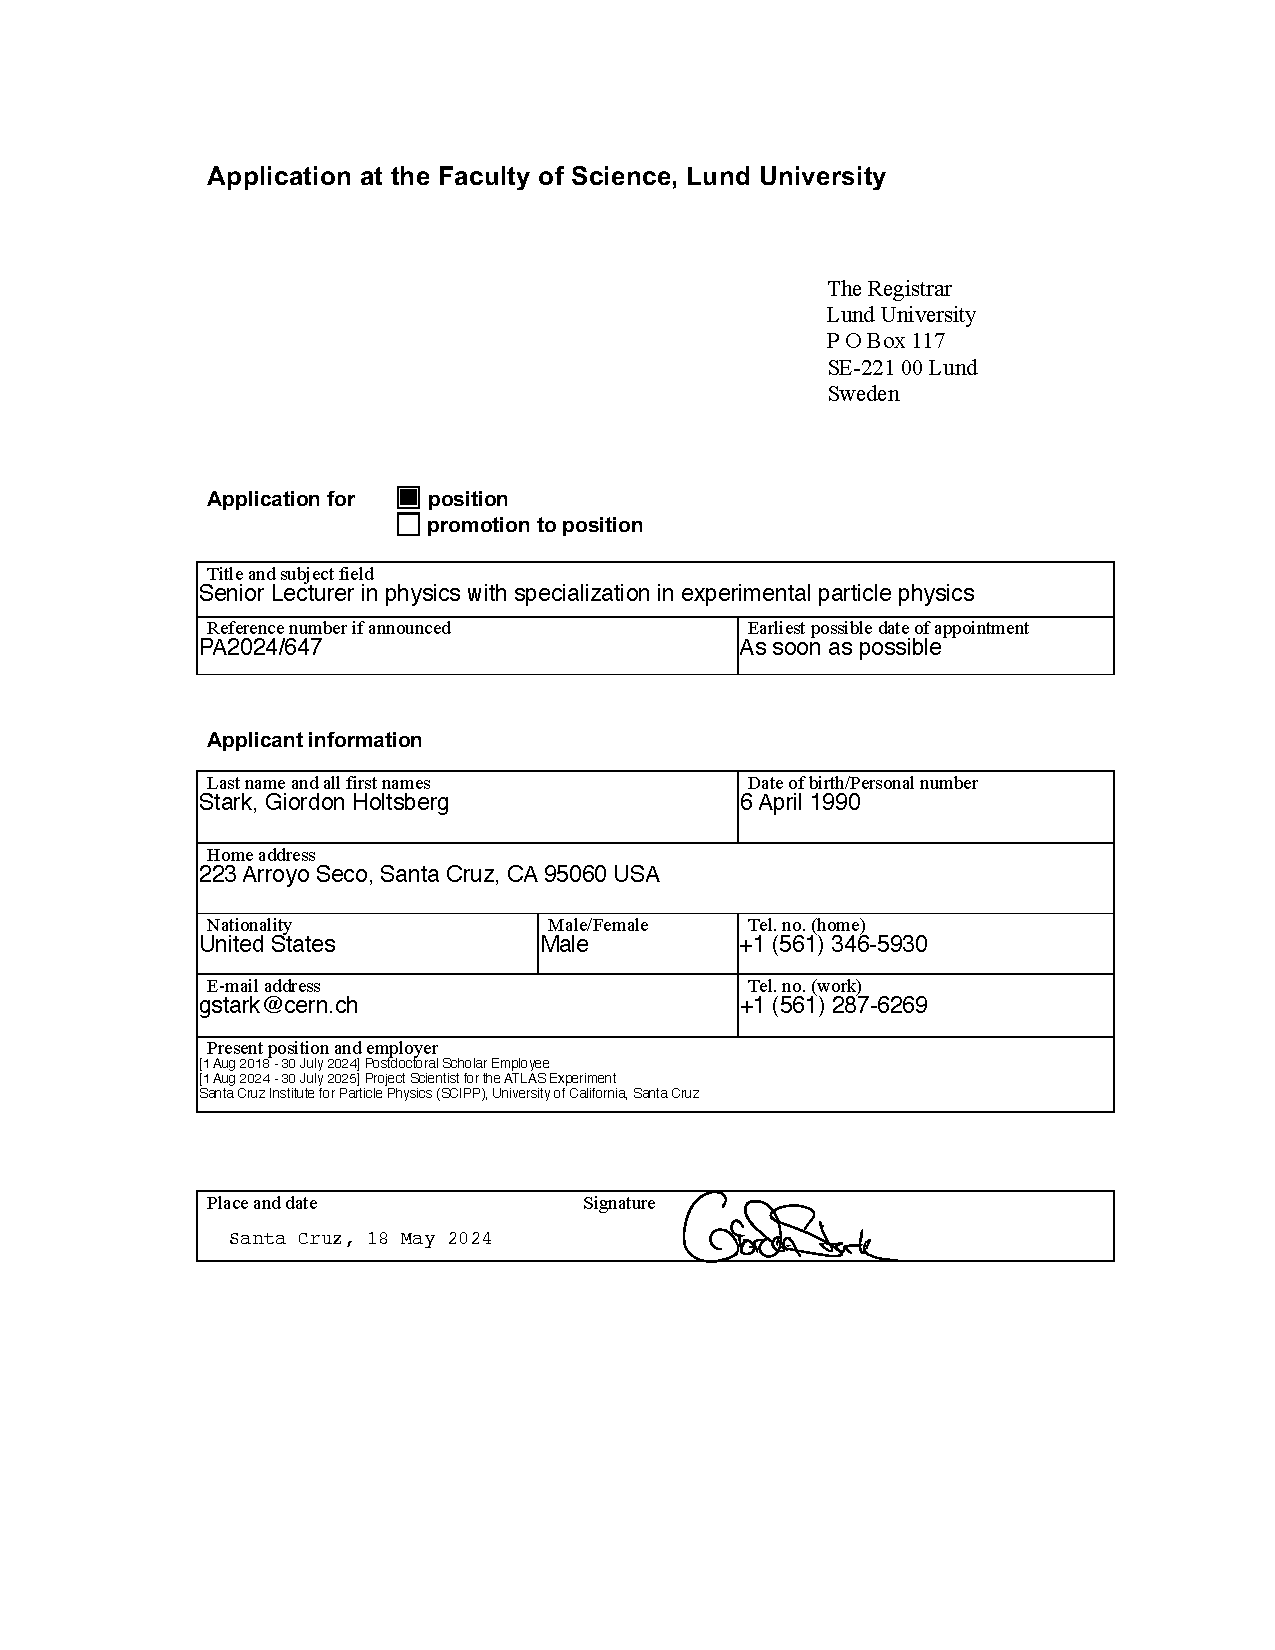
\includegraphics[width=1.1\textwidth]{attachments/cover-letter-academic-position-180928}}%

\clearpage
\section{Personal Letter} \label{sec:personal-letter}

\noindent Dear Prof. Lytken and the Lund Search Committee, \hfill \fcolorbox{black}{black!10}{May 25th, 2024}
\vspace{1em}

% TODO: maybe mention my leadership roles (ITk, Prod DB, FTF, DEI, etc)

I am attaching my application for the job position (\#PA2024/647) at Lunds universitet: \enquote{Universitetslektor i fysik med inriktning mot experimentell partikelfysik}. I found this position through a Swedish colleague. I obtained my Ph.D. in Physics from the University of Chicago in 2018 and am currently a postdoctoral scholar employee at the University of California, Santa Cruz, working on the ATLAS Experiment. Beginning August 1st, I transition to a Project Scientist position. I am thrilled at the prospect of continuing my work as a member of the ATLAS collaboration, my dedication to probing the fundamental questions of the Standard Model, and my passion for communicating my knowledge to Lund. My career in physics represents a commitment to the core value that Lund shares: widening participation for an inclusive University. In the attachments, I provide a diversity statement describing my unique background as a Deaf human in an oral world and how that shapes my passion for community outreach. And in both research and teaching, I work to provide a safe and inclusive environment so that my students, mentees, and colleagues can freely collaborate and foster new ideas. If appointed, my research program will be focused on Standard Model measurements, searches for new physics with the ATLAS experiment, instrumentation upgrades to support the completion of the HL-LHC physics program, and software development to meet the computing challenges of particle physics over the next decade.

At UChicago and UC Santa Cruz, I have been mentoring undergraduate students and graduate students across all of my research projects in hardware, software, and physics. Under my tutelage, I guided students through their physics analysis, supported them through struggles in their work-life balance, and worked with them to achieve their personal goals. For example, I was proud to mentor a graduate student, Dr. Jacob Pasner, who graduated from UCSC in 2019 with his Ph.D. on a search for boosted Higgs bosons. He finished his AAAS Fellowship in Washington, DC and now works for the State of California applying data science to water conservation efforts. I am also active in outreach activities, from giving international plenary talks to students in physics on how to advocate for their education and introducing LHC physics to local high schools through the QuarkNet and Masterclass programs. And finally, I was an active participant in the most recent Snowmass community effort to study the prospects of future colliders. My goal is to ensure a broad scope of work for myself and my students and continuity beyond the completion of the LHC program.

On a more personal note, one of the primary reasons for applying to this position is that I truly enjoyed the camaderie I experienced when I gave a seminar talk in September 2022 at your institution. I had a chance to talk with some of the current faculty there and appreciated the effort Lund invests in ensuring the success of all community members, both faculty and students alike. I feel that Lund will provide me the freedom to expand my current research activities and continue changing the status quo for modern particle physics, such as making ATLAS the first particle physics experiment to publish serialized, complete probability models for use by theorists, and as a teaching tool for statistics pedagogy.

Over the next decade, I plan to continue my close collaborations with various institutions and labs, including UChicago, UCSC, TUM, DESY, KTH, and IRIS-HEP, to support my research program. I am excited to keep working closely with the physics faculty and colleagues that I've worked with as a postdoc. As the first Deaf particle physicist, I am a very visual learner, and I have already been learning Swedish Sign Language for the past year. I am happy to provide any additional material upon request, in addition to the enclosed Academic Qualifications Portfolio.


\includegraphics[height=1cm]{attachments/signature}
\vfill%
